% -*- root: ../../main.tex -*-
\section{Design}

Come precedentemetne specificato, si è deciso di procedere allo sviiluppo del sistema utilizzando il paradigma ad attori. Durante la fase di progettazione sono state designate come attori le seguenti entità:

\begin{itemize}
	\item{\textbf{Client Actor:}} è l'attore che incapsula il comportamento del client 
	\item{\textbf{Server Actor:}} è l'attore che rappresenta il server e, in quanto tale, presenta tre diversi behaviour:
		\begin{itemize}
		 	\item{\textbf{Leader:}} quando un server è leader, svolge le seguenti mansioni:
		 		\begin{itemize}
					\item \emph{\textbf{accogliere} le richieste del client, che arriveranno tramite un messaggio opportuno.}
					\item \emph{\textbf{appenderle} al proprio log, al fine di accodarle per una futura esecuzione.}
					\item \emph{\textbf{propagare} le proprie entry verso gli altri server, allo scopo di replicare il proprio log su tutti i server.} 
					\item \emph{\textbf{committare} le entry quando diventa \textbf{safe} farlo}  
					\item \emph{\textbf{recedere} dal proprio ruolo di comando nel momento in cui si trova dinanzi a un poteziale nuovo leader, più qualificato.}
				\end{itemize}

		 	\item{\textbf{Follower:}} un server follower porta a termine i seguenti compiti:
		 		\begin{itemize}
					\item \emph{\textbf{appendere} le entry del leader al proprio log, quando quest'ultimo ordina di farlo.}
					\item \emph{\textbf{modificare} il proprio log, eliminando le entry non compatibili con quelle del leader, al fine di convergere al suo stesso stato}
					\item \emph{\textbf{committare} le entry quando il leader indica di farlo.}
					\item \emph{\textbf{ridirigere} il client, comunicando l'identità del leader, in caso si riceva una richiesta.}
					\item \emph{\textbf{votare} per i candidati che richiedono un voto, esprimendo un giudizio positivo o negativo, a seconda del soddisfacimento delle condizioni necessarie.} 					  
					\item \emph{\textbf{candidarsi} come potenziale leader nel momento in cui si perdono i contatti con quello corrente e si assume, di conseguenza, che sia attualmente irraggiungibile.}
				\end{itemize}
		 	\item{\textbf{Candidate:}} un server in modalità candidato esegue le seguenti operazioni:
		 		\begin{itemize}
					\item \emph{\textbf{inviare} richieste di voto agli altri server}
					\item \emph{\textbf{contare} le risposte positive e cambiare il proprio stato in \textbf{leader} in caso di maggioranza dei voti.}
					\item \emph{\textbf{recedere} a \textbf{follower} nel caso in cui le elezioni siano vinte da qualcun altro}
					\item \emph{\textbf{ricandidarsi} una seconda volta nel caso in cui, allo scadere di un timer, non si sia raggiunta la maggioranza dei voti nè si sia venuti a conoscenza dell'avvenuta elezione di un nuovo leader.} 					  
					
				\end{itemize}
		 \end{itemize} 
	\item{\textbf{State Machine:}} è un attore figlio del Server Actor e incapsula la gestione delle richieste da eseguire e la restituzione del risultato.
\end{itemize}




This is where the logical / abstract contribution of the project is presented.

Notice that, when describing a software project, three dimensions need to be taken into account: structure, behaviour, and interaction.

Always remember to report \textbf{why} a particular design has been chosen.
Reporting wrong design choices which has been evalued during the design phase is welcome too.

\subsection{Struttura}

Which entities need to by modelled to solve the problem?
%
(UML Class diagram)

\begin{figure}[H]
  \centering
  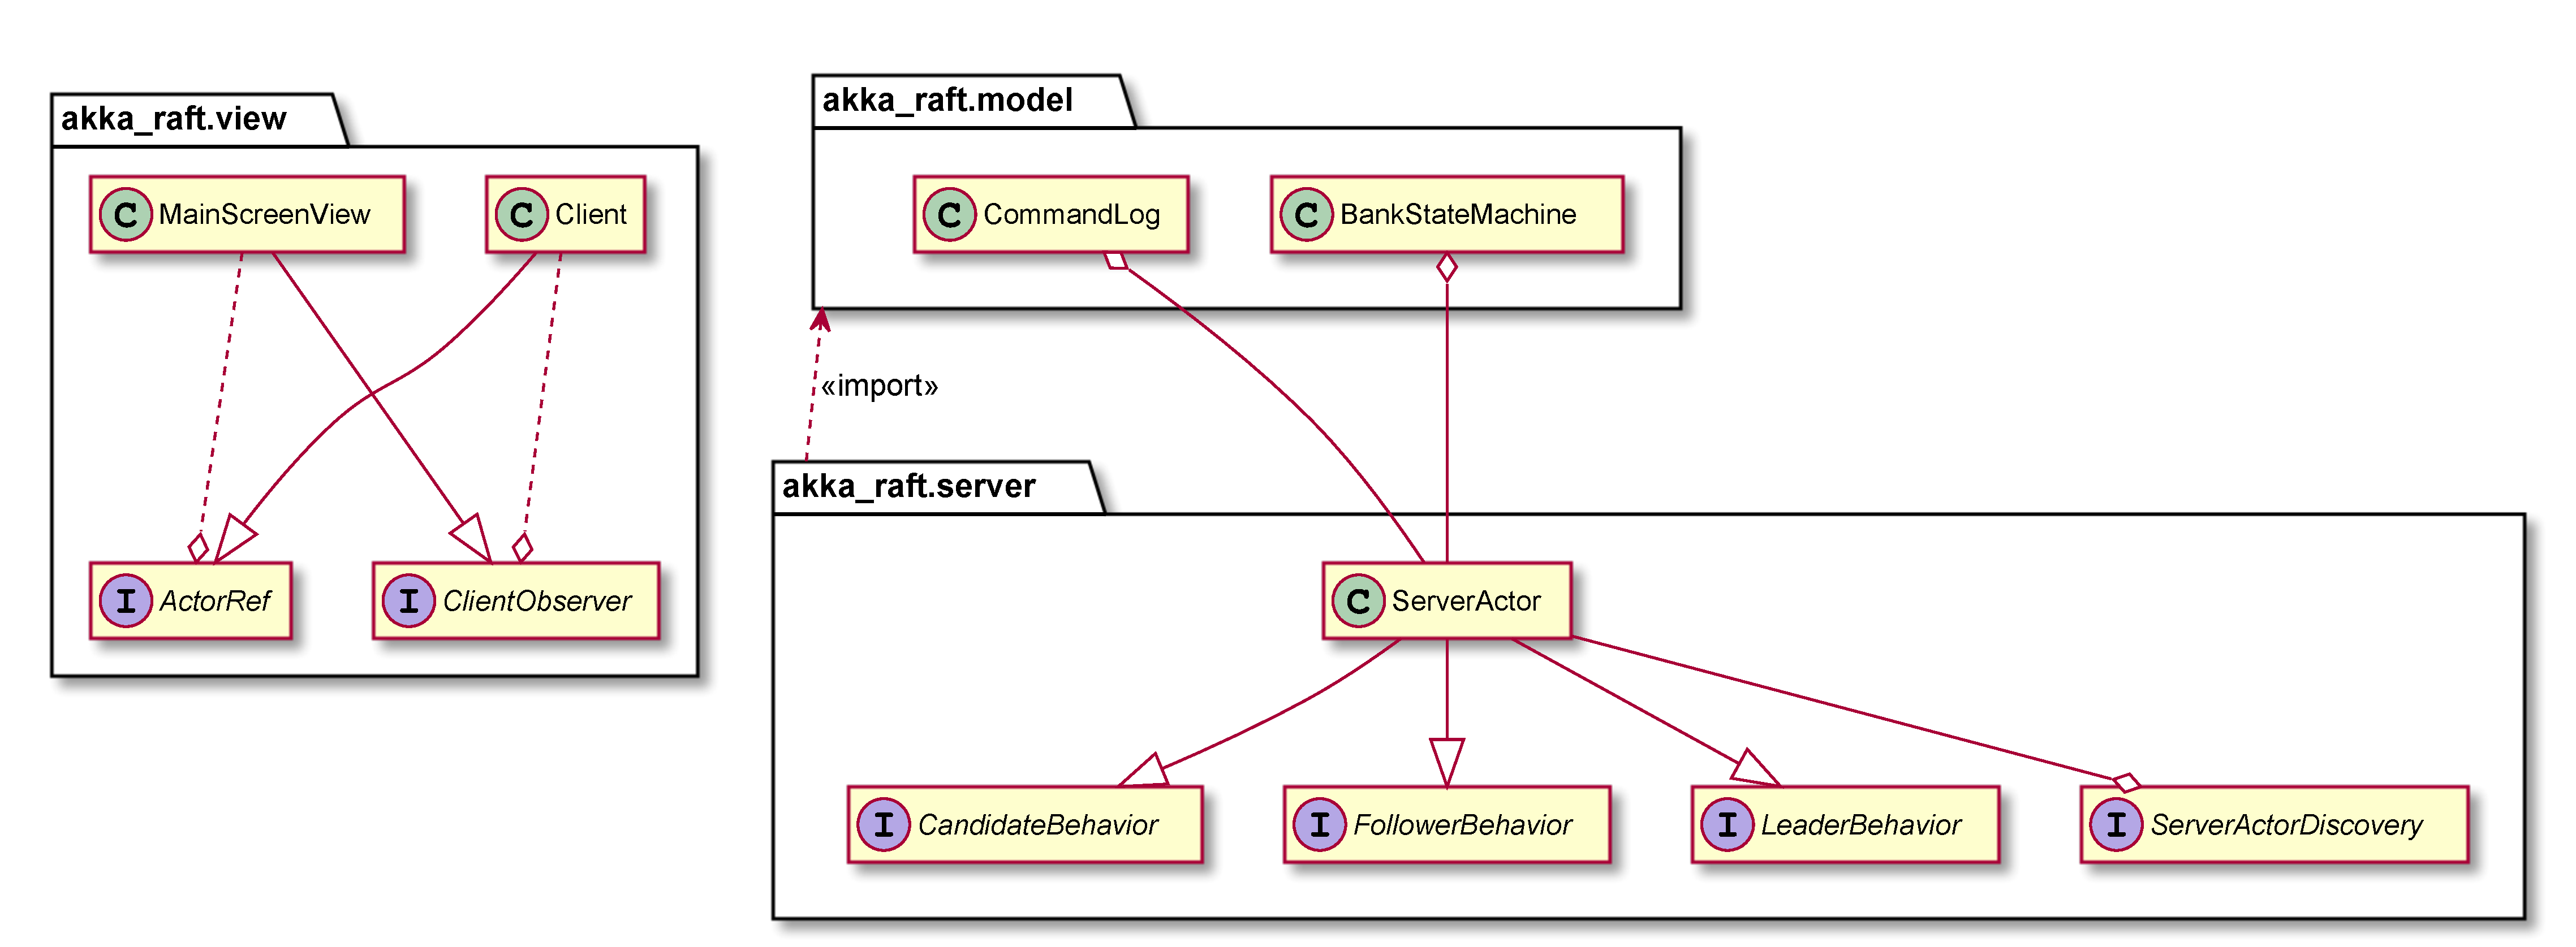
\includegraphics[width=0.99\columnwidth]{classDiagrams/classDiagram}
  \caption[classDiagramCaption]{}
  
  \label{fig:figure29}
\end{figure}

How should entities be modularised?
%
(UML Component / Package / Deployment Diagrams)

\begin{figure}[H]
  \centering
  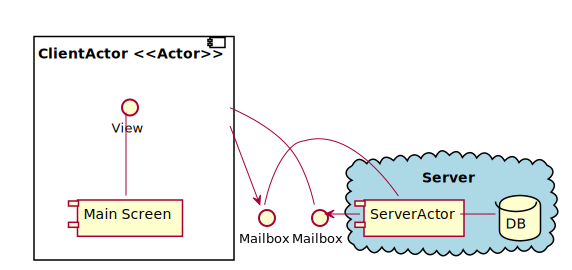
\includegraphics[width=0.99\columnwidth]{componentDiagrams/componentDiagram}
  \caption[componentDiagramCaption]{}
  
  \label{fig:figure30}
\end{figure}

\subsection{Comportamento}

How should each entity behave?
%
(UML State diagram or Activity Diagram)

\subsection{Interazione}

How should entities interact with each other?
%
(UML Sequence Diagram)
